% % includemthe figures path relative to the master file
% \graphicspath{ {./content/other/figures/} }

% \section{other}
% \label{sec:other}  % \label{} allows reference to this section

% This section is used testing that the packages perform as expected regardless of the template in hand.

% \subsection{General}
% \label{sec:other:general}
% Here is some text referencing some \cref{eq:simple_equation} and \cref{fig:simulationfigure}.

% \begin{equation}
%     \label{eq:simple_equation}
%     \alpha = \sqrt{ \beta }
% \end{equation}

% \begin{figure}
%     \centering
%     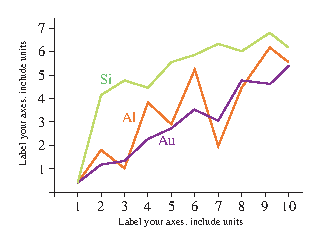
\includegraphics[width=3.0in]{fig_1}
%     \caption{Simulation Results}
%     \label{fig:simulationfigure}
% \end{figure}

% \subsection{Citations}
% \label{sec:other:citations}
% % This file is an addaptation of the biblatex citation example that can be
% found at:
%   http://www.ctan.org/tex-archive/macros/latex/contrib/biblatex/doc/examples/
%
% The example uses the database biblatex-examples.bib.
% \addbibresource{biblatex-examples.bib}
%
% Some generic settings.
\newcommand{\cmd}[1]{\texttt{\textbackslash #1}}
\setlength{\parindent}{0pt}

This section adapts this
\href{http://www.ctan.org/tex-archive/macros/latex/contrib/biblatex/doc/examples/01-introduction.tex}{example}
in order to illustrate the usage of the \emph{biblatex} package with a biber backend.
Dudring the development of the document, the bibligraphic style is recomended to be set up as \textbf{draf}
(see this \href{http://mirrors.ircam.fr/pub/CTAN/macros/latex/contrib/biblatex/doc/examples/81-style-draft.pdf}{example}).
The full \emph{biblatex} documentation can be found \href{http://www.ctan.org/pkg/biblatex}{here}.

\begin{description}
  \item [Style-dependent] \cmd{cite} \cmd{parencite} \cmd{footcite} \cmd{textcite}
  \item [Sytle-independent] \cmd{autocite}
  \item [Text ingegrated] \cmd{citeauthor} \cmd{citetitle} \cmd{citetitle*} \cmd{citeyear}
  \item [Special] \cmd{nocite} \cmd{fullcite} \cmd{footfullcite}
\end{description}

\subsubsection*{The \cmd{cite} command}

Prints a bare citation without parentheses, that can be called
as it is, \cmd{cite\{key\}} producing \cite{companion};
~$\cdot$~
indicating a reference page (or range) \cmd{cite[59]\{key\}} producing \cite[59]{companion};
~$\cdot$~
with a note \cmd{cite[see][]\{companion\}} producing \cite[see][]{companion};
~$\cdot$~
or both \cmd{cite[see][59--63]\{companion\}} \cite[see][59--63]{companion}.

\subsubsection*{The \cmd{parencite} command}

This command, which is intended for in-text citations,
encloses the citation in parentheses. Note that the 'numeric' and
'alphabetic' styles use square brackets instead.
Like before it can be called as it is, \cmd{parencite\{key\}} producing \parencite{companion};
~$\cdot$~
indicating a reference page (or range) \cmd{parencite[59]\{key\}} producing \parencite[59]{companion};
~$\cdot$~
with a note \cmd{parencite[see][]\{companion\}} producing \parencite[see][]{companion};
~$\cdot$~
or both \cmd{parencite[see][59--63]\{companion\}} \parencite[see][59--63]{companion}.

\subsubsection*{The \cmd{footcite} command}

is similar to \cmd{parencite}, except that the
citation is given in a footnote.
It can be called as it is, \cmd{footcite\{key\}} producing \footcite{companion};
~$\cdot$~
indicating a reference page (or range) \cmd{footcite[59]\{key\}} producing \footcite[59]{companion};
~$\cdot$~
with a note \cmd{footcite[see][]\{companion\}} producing \footcite[see][]{companion};
~$\cdot$~
or both \cmd{footcite[see][59--63]\{companion\}} \footcite[see][59--63]{companion}.

\subsubsection*{The \cmd{textcite} command}

is intended for citations integrated in the
flow of text, replacing the subject of the sentence.

\textcite{companion} show that this is just filler text called as
\cmd{texcite\{key\}}, which can also be called with a parameter
\cmd{textcite[59]\{key\}} to produce \textcite[59]{companion} showing
that this is just filler text.

With \cmd{textcite}, the first optional argument is of limited use
only, since you could simply place the prenote in front of the
citation. It is still supported for the sake of consistency.

\textcite[see][]{companion} show that this is just filler text
produced by \cmd{textcite[see][]\{companion\}}
while \cmd{textcite[see][59--63]\{companion\}} produces
\textcite[see][59--63]{companion} plus some text filler.


\subsubsection*{The \cmd{autocite} command}

The point of the \cmd{autocite} command is that it automatically adapts
to the predominant citation format (inline or footnote) normally
used with the selected citation style. It should be used at the
end of the sentence and usually works like \cmd{parencite} or
\cmd{footcite}, depending on the citation style and the setting of the
'autocite' package option. With the author-year style used in this
example, it works like \cmd{parencite}:

This is just filler text \autocite{companion}.

\subsubsection*{Text commands}

There are a few predefined commands for bibliographic data which
is frequently used in the flow of text. 
Like \cmd{citeauthor} to recall the author, \cmd{citetitle} for
the short-title when available, \cmd{citetitle*} for the full title, 
or \cmd{citeyear} to retrieve the year.

\citetitle*{companion} by \citeauthor{companion} was
published in \citeyear{companion} has the following short-title:
\citetitle{companion}.

Note that biblatex also grants access to all lists and fields at a lower level,
see documentation.


% \subsection{Acronyms}
% \label{sec:other:acro}
% %
% This are some examples using the acro package.

Example showing how plurals are easily handeled:
\\
first time: \ac{a} \\
second time: \ac{a} \\
short: \acs{a} \\
alternative: \aca{a} \\
first again: \acf{a} \\
long: \acl{a} \\
short plural: \acsp{a} \\
long plural: \aclp{a} \\

Here is an example of this \href{}{acro package}
using nested declarations and macro-acronyms calls, taken from
\href{http://tex.stackexchange.com/questions/135975/how-to-define-an-acronym-by-using-other-acronym-and-print-the-abbreviations-toge}{stackOverflow}.

\subsubsection*{nested acronyms example 1}

\Ac{dna} is a very important molecule.  The virus xyz contains \dsdna.  Apart
from that, \dna exists in almost all cells of the body. In most cases it is
\dsdna.

\subsubsection*{nested acronyms example 2}
\acresetall

The virus xyz contains \dsdna.  \Ac{dna} is a very important molecule.  Apart
from that, \dna exists in almost all cells of the body. In most cases it is
\dsdna.


% You may title this section "Methods" or "Models". 
% "Models" is not a valid title for PLoS ONE authors. However, PLoS ONE
% authors may use "Analysis" 
\section*{Materials and Methods}
\subsection*{Etiam eget sapien nibh.}

% For figure citations, please use "Fig." instead of "Figure".
Nulla mi mi, Fig.~\ref{fig1} venenatis sed ipsum varius, volutpat euismod diam. Proin rutrum vel massa non gravida. Quisque tempor sem et dignissim rutrum. Lorem ipsum dolor sit amet, consectetur adipiscing elit. Morbi at justo vitae nulla elementum commodo eu id massa. In vitae diam ac augue semper tincidunt eu ut eros. Fusce fringilla erat porttitor lectus cursus, \nameref{S1_Video} vel sagittis arcu lobortis. Aliquam in enim semper, aliquam massa id, cursus neque. Praesent faucibus semper libero.

\begin{figure}[h]
\caption{{\bf Figure Title first bold sentence Nulla mi mi, venenatis sed ipsum varius, volutpat euismod diam.}
Figure Caption Proin rutrum vel massa non gravida. Quisque tempor sem et dignissim rutrum. A: Lorem ipsum dolor sit amet. B: Consectetur adipiscing elit.}
\label{fig1}
\end{figure}

\begin{enumerate}
\item{react}
\item{diffuse free particles}
\item{increment time by dt and go to 1}
\end{enumerate}

% Results and Discussion can be combined.
\section*{Results}
Nulla mi mi, venenatis sed ipsum varius, Table~\ref{table1} volutpat euismod diam. Proin rutrum vel massa non gravida. Quisque tempor sem et dignissim rutrum. Lorem ipsum dolor sit amet, consectetur adipiscing elit. Morbi at justo vitae nulla elementum commodo eu id massa. In vitae diam ac augue semper tincidunt eu ut eros. Fusce fringilla erat porttitor lectus cursus, vel sagittis arcu lobortis. Aliquam in enim semper, aliquam massa id, cursus neque. Praesent faucibus semper libero.


\begin{table}[!ht]
\begin{adjustwidth}{-2.25in}{0in} % Comment out/remove adjustwidth environment if table fits in text column.
\caption{
{\bf Table caption Nulla mi mi, venenatis sed ipsum varius, volutpat euismod diam.}}
\begin{tabular}{|l|l|l|l|l|l|l|l|}
\hline
\multicolumn{4}{|l|}{\bf Heading1} & \multicolumn{4}{|l|}{\bf Heading2}\\ \hline
$cell1 row1$ & cell2 row 1 & cell3 row 1 & cell4 row 1 & cell5 row 1 & cell6 row 1 & cell7 row 1 & cell8 row 1\\ \hline
$cell1 row2$ & cell2 row 2 & cell3 row 2 & cell4 row 2 & cell5 row 2 & cell6 row 2 & cell7 row 2 & cell8 row 2\\ \hline
$cell1 row3$ & cell2 row 3 & cell3 row 3 & cell4 row 3 & cell5 row 3 & cell6 row 3 & cell7 row 3 & cell8 row 3\\ \hline
\end{tabular}
\begin{flushleft} Table notes Phasellus venenatis, tortor nec vestibulum mattis, massa tortor interdum felis, nec pellentesque metus tortor nec nisl. Ut ornare mauris tellus, vel dapibus arcu suscipit sed.
\end{flushleft}
\label{table1}
\end{adjustwidth}
\end{table}



\subsection*{\lorem\ and \ipsum\ Nunc blandit a tortor.}

Maecenas convallis mauris sit amet sem ultrices gravida. Etiam eget sapien nibh. Sed ac ipsum eget enim egestas ullamcorper nec euismod ligula. Curabitur fringilla pulvinar lectus consectetur pellentesque. Quisque augue sem, tincidunt sit amet feugiat eget, ullamcorper sed velit. Sed non aliquet felis. Lorem ipsum dolor sit amet, consectetur adipiscing elit. Mauris commodo justo ac dui pretium imperdiet. Sed suscipit iaculis mi at feugiat. 

\subsection*{Sed ac quam id nisi malesuada congue.}

Nulla mi mi, venenatis sed ipsum varius, volutpat euismod diam. Proin rutrum vel massa non gravida. Quisque tempor sem et dignissim rutrum. Lorem ipsum dolor sit amet, consectetur adipiscing elit. Morbi at justo vitae nulla elementum commodo eu id massa. In vitae diam ac augue semper tincidunt eu ut eros. Fusce fringilla erat porttitor lectus cursus, vel sagittis arcu lobortis. Aliquam in enim semper, aliquam massa id, cursus neque. Praesent faucibus semper libero.

% Please do not create a heading level below \subsection. For 3rd level headings, use \paragraph{}. 
\subsection*{Subsection 1}
Nulla mi mi, venenatis sed ipsum varius, volutpat euismod diam. Proin rutrum vel massa non gravida. Quisque tempor sem et dignissim rutrum. Lorem ipsum dolor sit amet, consectetur adipiscing elit. Morbi at justo vitae nulla elementum commodo eu id massa. In vitae diam ac augue semper tincidunt eu ut eros. Fusce fringilla erat porttitor lectus cursus, vel sagittis arcu lobortis. Aliquam in enim semper, aliquam massa id, cursus neque. Praesent faucibus semper libero.

\subsection*{Subsection 2}
\paragraph{3rd Level Heading.} Nulla mi mi, venenatis sed ipsum varius, volutpat euismod diam. Proin rutrum vel massa non gravida. Quisque tempor sem et dignissim rutrum. Lorem ipsum dolor sit amet, consectetur adipiscing elit. Morbi at justo vitae nulla elementum commodo eu id massa. In vitae diam ac augue semper tincidunt eu ut eros. Fusce fringilla erat porttitor lectus cursus, vel sagittis arcu lobortis. Aliquam in enim semper, aliquam massa id, cursus neque. Praesent faucibus semper libero.

\section*{Discussion}
Nulla mi mi, venenatis sed ipsum varius, Table~\ref{table1} volutpat euismod diam. Proin rutrum vel massa non gravida. Quisque tempor sem et dignissim rutrum. Lorem ipsum dolor sit amet, consectetur adipiscing elit. Morbi at justo vitae nulla elementum commodo eu id massa. In vitae diam ac augue semper tincidunt eu ut eros. Fusce fringilla erat porttitor lectus cursus, vel sagittis arcu lobortis. Aliquam in enim semper, aliquam massa id, cursus neque. Praesent faucibus semper libero.

\subsection*{\lorem\ and \ipsum\ Nunc blandit a tortor.}

CO\textsubscript{2} Maecenas convallis mauris sit amet sem ultrices gravida. Etiam eget sapien nibh. Sed ac ipsum eget enim egestas ullamcorper nec euismod ligula. Curabitur fringilla pulvinar lectus consectetur pellentesque. Quisque augue sem, tincidunt sit amet feugiat eget, ullamcorper sed velit. 

Sed non aliquet felis. Lorem ipsum dolor sit amet, consectetur adipiscing elit. Mauris commodo justo ac dui pretium imperdiet. Sed suscipit iaculis mi at feugiat. Ut neque ipsum, luctus id lacus ut, laoreet scelerisque urna. Phasellus venenatis, tortor nec vestibulum mattis, massa tortor interdum felis, nec pellentesque metus tortor nec nisl. Ut ornare mauris tellus, vel dapibus arcu suscipit sed. Nam condimentum sem eget mollis euismod. Nullam dui urna, gravida venenatis dui et, tincidunt sodales ex. Nunc est dui, sodales sed mauris nec, auctor sagittis leo. Aliquam tincidunt, ex in facilisis elementum, libero lectus luctus est, non vulputate nisl augue at dolor. For more information, see \nameref{S1_Text}.

\section*{Supporting Information}

% Include only the SI item label in the subsection heading. Use the \nameref{label} command to cite SI items in the text.
\subsection*{S1 Video}
\label{S1_Video}
{\bf Bold the first sentence.}  Maecenas convallis mauris sit amet sem ultrices gravida. Etiam eget sapien nibh. Sed ac ipsum eget enim egestas ullamcorper nec euismod ligula. Curabitur fringilla pulvinar lectus consectetur pellentesque.

\subsection*{S1 Text}
\label{S1_Text}
{\bf Lorem Ipsum.} Maecenas convallis mauris sit amet sem ultrices gravida. Etiam eget sapien nibh. Sed ac ipsum eget enim egestas ullamcorper nec euismod ligula. Curabitur fringilla pulvinar lectus consectetur pellentesque.

\subsection*{S1 Fig}
\label{S1_Fig}
{\bf Lorem Ipsum.} Maecenas convallis mauris sit amet sem ultrices gravida. Etiam eget sapien nibh. Sed ac ipsum eget enim egestas ullamcorper nec euismod ligula. Curabitur fringilla pulvinar lectus consectetur pellentesque.

\subsection*{S2 Fig}
\label{S2_Fig}
{\bf Lorem Ipsum.} Maecenas convallis mauris sit amet sem ultrices gravida. Etiam eget sapien nibh. Sed ac ipsum eget enim egestas ullamcorper nec euismod ligula. Curabitur fringilla pulvinar lectus consectetur pellentesque.

\subsection*{S1 Table}
\label{S1_Table}
{\bf Lorem Ipsum.} Maecenas convallis mauris sit amet sem ultrices gravida. Etiam eget sapien nibh. Sed ac ipsum eget enim egestas ullamcorper nec euismod ligula. Curabitur fringilla pulvinar lectus consectetur pellentesque.


% Some stuff that emac's colegues use
%%% Local Variables:
%%% mode: late
%%% TeX-master: "../../master.tex"
%%% End: \section{other}

